\documentclass[12pt]{article} \usepackage[a4paper,margin=1in]{geometry} \usepackage{amsmath,amssymb,amsthm} \usepackage{graphicx} \usepackage{hyperref} \usepackage{booktabs} \usepackage{enumitem} \usepackage{natbib} \usepackage{microtype} \usepackage{tabularx} \usepackage{array} \usepackage{caption} \usepackage{xcolor} \usepackage{tikz} \usetikzlibrary{arrows.meta,positioning} \title{Intelligent Networks: A Viability Framework with Axioms, Metrics, and Tests} \author{Albert Jan van Hoek \and [Second Author, if any]} \date{\today} \newtheorem{definition}{Definition} \newtheorem{axiom}{Axiom} \newtheorem{proposition}{Proposition} \begin{document} \renewcommand{\arraystretch}{1.2} \setlength{\tabcolsep}{6pt} \maketitle \begin{abstract}We ask whether a \emph{scientific}, \emph{instrumental} answer (viability under uncertainty) to the perennial `meaning of life'' question is possible. We recast it as: \emph{How should a single node act so that the network it depends on becomes more resilient, more robust, more longer living?} We pre-register adequacy criteria (falsifiability, operational clarity, predictive/retrodictive adequacy, reproducibility, corrigibility, local actionability, ethical floors, second-order stability) and use an abductive--deductive--inductive loop. From basic facts (mortality/entropy; lack of innate knowledge; structural interdependence; uncertainty/shocks; heterogeneity and the need for translation; bounded rationality; intergenerational horizons) we \emph{deduce} the minimal mechanism: an \emph{intelligent network} of agents with explicit substrates, typed edges (information, incentive/reciprocity, stewardship, translation), and embedded feedback/review. This yields viability axioms and operational indices (EEI, $EH=\langle p,a,d,\lambda,r\rangle$, AHI, dominance $D$, MTTR, translation fidelity $\tau$), with falsifiable hypotheses (H1--H8) spanning simulations, human teams, multi-agent AI, and quasi-experiments. Under weak monotonicity of the viability functional $\mathcal V$, a single instrumental aim emerges: \emph{keep alive what keeps us alive---and improve it across generations}. We discuss measurement and causal challenges, threat models, and guardrails. Our contribution is not metaphysics but a testable, corrigible programme: design levers (edge repair, translation-first coupling, stewardship for conditional nodes, calibrated dominance windows, review topologies) that align ego-level action with network-level resilience.\end{abstract} \end{abstract} \section{Introduction and origin} \n\paragraph{Working definition.} An \emph{intelligent network} is a system of agents that (i) update beliefs from evidence, (ii) act on and help maintain their substrates, and (iii) propagate corrective frameworks via review and translation edges.\n\n\paragraph{Research gap and thesis.} Existing strands in sociology/organizational science and AI teamwork typically lack (a) edge-primacy metrics on typed edges (EQ), (b) cross-substrate translation fidelity $\tau$, and (c) Goodhart-aware governance embedded as first-class design. We contribute a testable viability framework that supplies these hooks.\n\n\emph{Reader's map.} Section~2 states criteria and method; Section~3 derives minimal structure; Section~4 gives viability conditions; Section~5 defines indices; Section~6–7 provide scenarios and hypotheses; Sections~8–10 cover ethics, limitations, and open questions.\n \subsection*{Scope and contribution (reader's map)} We treat `meaning'' instrumentally as \emph{viability under uncertainty}. The contribution is technical: (i) derive a minimal intelligent-network structure from basic facts; (ii) state viability conditions (axioms); (iii) define operational indices (EEI, $EH$, AHI, $D$, MTTR, $\tau$); (iv) pose falsifiable hypotheses and study designs. Philosophical inspiration motivates the question, but claims are restricted to intelligent networks; metaphysical theses are out of scope. We interpret `meaning'' instrumentally: actions that raise network viability under uncertainty, subject to ethical safety floors. \nThis paper starts from a simple, difficult question: \emph{What should I do that truly helps?} We ask whether such big questions of life can be reformulated as a scientific question about practice: \emph{how can a single person (or agent) act so that the whole becomes wiser, faster, and more resilient?} Our premise is modest but powerful: small, local choices—how we connect, how we share, how we translate across viewpoints and tools, and how we care for what our work rests on—can add up to reliable improvements in what groups can do together. This reframing targets a timeless concern about purpose and agency, treating it as something we can observe, compare, and improve rather than settle by decree.\n\n\paragraph{Research gap and thesis.}\nWe lack a common, testable way to connect personal action under overwhelm to improvements in collective capability. Our thesis is that this gap can be closed by treating purpose as empirical practice: identify local actions whose effects on group learning, fairness of access, and safe responsibility are \emph{measurable and replicable}—and study what changes when many people do the same.\n\n\paragraph{What follows.}\nWe provide a simple vocabulary and viability conditions, then introduce operational measures and falsifiable hypotheses. Details on networks and metrics arrive only as needed. The aim is not to settle the meaning of life, but to make \emph{meaningful action} observable, comparable, and improvable—and to show how second-order collaboration emerges when this practice scales.\n\n\paragraph{Scope note.}\nWe do not claim a single, universal `meaning of life.'' Our contribution is narrower and practical: a way to study how individual actions can reliably improve shared capability—across contexts and cultures—so that a perennial question becomes a programme for inquiry and practice.\n \paragraph{Contributions.} (i) Formal definitions for intelligent networks, nodes/edges, substrates and conditional nodes, edge quality, and epistemic health; (ii) nine axioms that specify viability conditions (interdependence, edge primacy, node integrity, epistemic health, self-awareness, dynamic alignment, balanced dynamics, reflexive propagation, agency); (iii) operational measures (edge quality and epistemic health vectors) and an agency health index; (iv) illustrative scenarios spanning human science, AI multi-agent systems, and substrate-agnostic cases; and (v) testable predictions and an agenda for simulations and field studies. \paragraph{Scope.} This is a conceptual discussion paper: we aim to sharpen vocabulary, isolate assumptions, and provide measurable hooks for subsequent formalization and empirical work. We do not claim a unique foundation; rather, we assemble and extend existing insights to the special case of networks whose components can intentionally reshape the networks that sustain them. \paragraph{Why this matters.} Focusing on intelligent networks isolates conditions under which self-aware agents can sustain themselves and the systems they inhabit, revealing levers (edges, epistemic health, stewardship) that general network models overlook. \par\smallskip We operationalize what counts as a \emph{scientific answer} via pre-registered criteria. We then derive a minimal network structure from basic facts, from which the practical aim follows instrumentally. \section{Methods} \begin{figure}[h] \centering \begin{tabular}{c} \large \textbf{Basic facts (P1--P7)} \\ $\Downarrow$ \\ \large \textbf{Necessary structure (intelligent network)} \\ $\Downarrow$ \\ \large \textbf{Viability conditions (axioms)} \\ $\Downarrow$ \\ \large \textbf{Operational indices (EEI, $EH$, AHI, $D$, MTTR, $\tau$)} \\ $\Downarrow$ \\ \large \textbf{Testable hypotheses (H1--H9) \& designs (S1--S4)} \end{tabular} \caption{Pipeline from basic facts to tests. Acronyms: EEI (Epistemic Equality Index), EH (epistemic health vector), AHI (Agency Health Index), D (dominance), MTTR (mean time-to-recovery), $\tau$ (translation fidelity).} \end{figure} \subsection*{Assumption ledger and falsifiable implications} \begin{table}[h] \centering \small \begin{tabular}{p{4.0cm} p{6.5cm} p{6.8cm}} \hline \textbf{Assumption} & \textbf{Scope / likely failures} & \textbf{Falsifiable implication (link to H\#)} \\ \hline Weak monotonicity of $\mathcal V$ & Holds when EQ improves on critical edges and latency remains below tolerance; can fail under severe bottlenecks or mis-specified $D$ & If EQ on translation edges is randomly increased, MTTR decreases under OOD shocks (H1,H6) \\ Bounded-rational updating (correctable) & Humans under stress, incentives; misaligned AI & Protected critique increases accuracy without catastrophic latency (H3) \\ Dominance window $D$ mid-range & Too low: paralysis; too high: fragility & Networks with $D$ in mid-range show smaller cascade tails than low/high $D$ (H1) \\ Measurement proxies (EEI,$EH^\*$,AHI) are informative & Goodhart risks; construct drift & Metric rotation/adversarial audits reduce incident rates vs. static metrics (H5) \\ Stewardship enforceable for conditional nodes & Power asymmetries, capture & Stewardship contracts reduce MTTR after substrate shocks (H4) \\ \hline \end{tabular} \caption{Assumptions, where they may fail, and concrete disconfirmations.} \end{table} \subsection*{Viability functional $\mathcal V$ (minimal form)} Let $\mathcal{G}$ denote intelligent-network states and $\Theta$ design/control parameters (e.g., edge weights, review topology). We define a viability functional $\mathcal V:\mathcal{G}\times\Theta\to\mathbb{R}$ that scores persistence under uncertainty (higher is better), monotone in (i) edge quality on critical cuts and (ii) epistemic health $EH^\*$, holding latency within tolerance. \emph{Disconfirmation example.} If randomized increases of translation-edge EQ do \emph{not} reduce MTTR after OOD shocks (H1,H6), or if mid-range dominance $D$ \emph{increases} cascade tails, the assumed monotonicities fail; axioms or measurement must be revised. \subsection{A priori adequacy criteria} We count an answer as \emph{scientific} if it satisfies: \begin{enumerate} \item \textbf{Falsifiable \& testable} (pre-specified disconfirmation tests, thresholds). \item \textbf{Operational clarity} (named observables and feasible levers). \item \textbf{Predictive \& retrodictive adequacy} (explains past; forecasts with error bars). \item \textbf{Reproducible \& robust} (across contexts, under stress/OOD). \item \textbf{Corrigible} (assumptions explicit; versioned updates to evidence). \item \textbf{Local actionability} (ego-level steps with observable feedback). \item \textbf{Ethical safety floors} (agency, proportionality, reciprocity, transparency). \item \textbf{Second-order stability} (resistant to gaming; guardrails in place). \end{enumerate} We evaluate our result against this checklist in Section~\ref{sec:criteria-eval}. \subsection{Methodological stance: abductive--deductive--inductive loop} We discover (\emph{abduction}) recurring patterns and propose minimal structure; we formalize (\emph{deduction}) primitives, axioms, and derived claims; we test (\emph{induction}) with pre-registered hypotheses across simulations, human teams, and multi-agent AI, updating when evidence conflicts. \emph{Standing assumption:} bounded-rational updating, correctable via feedback and review. \subsection{From basic facts to necessary structure (deductive pathway)} \paragraph{Premises (basic facts).} \begin{enumerate} \item \textbf{Mortality \& entropy:} substrates (bodies, compute, energy, logistics) degrade; maintenance is required. \item \textbf{No innate propositional knowledge:} individuals must learn; external memory/transfer are needed. \item \textbf{Interdependence:} no individual supplies all resources or manages all risks at scale. \item \textbf{Uncertainty \& shocks:} stochastic environments demand redundancy and feedback control. \item \textbf{Heterogeneity \& translation:} sensors, languages, tools, norms differ; mutual intelligibility is non-trivial. \item \textbf{Bounded rationality:} bias/noise/incentives create systematic error unless correction channels exist. \item \textbf{Intergenerational horizon:} many aims/risks exceed one lifespan; cumulative retention and stewardship are required. \end{enumerate} \paragraph{Structural inferences.} \begin{enumerate} \item \textbf{Substrate stewardship is necessary} (P1, P3, P4). \item \textbf{Edges are primary carriers of viability} (P2--P6). \item \textbf{Feedback/peer-review is necessary} (P2, P4, P6). \item \textbf{Translation edges are necessary} (P5). \item \textbf{Conditional nodes arise; stewardship duty follows} (P1, P3). \item \textbf{Viability must be operationalised} (P2--P7): EEI, $EH=\langle p,a,d,\lambda,r\rangle$, AHI, $D$, MTTR, $\tau$. \end{enumerate} \paragraph{Minimal adequate structure.} An \emph{intelligent network} with explicit substrates, typed edges (information, incentive/reciprocity, stewardship, translation), and embedded feedback/review. Axioms in Section~\ref{sec:axioms}. % TODO: Consider pruning repetitions to 30--40% length. \section{Background and related work} \noindent\textit{Scope note.} We summarise key strands relevant to our claims; duplications and peripheral debates are omitted for concision. \paragraph{Emergence and hierarchical organization.} Anderson’s dictum that `more is different'' established that higher-level organization requires its own concepts and regularities \citep{Anderson1972}. Simon’s account of near-decomposable hierarchies explains how complex systems stabilize through modular structure \citep{Simon1962}. Kauffman’s NK-models and autocatalytic sets further showed how rugged fitness landscapes and self-sustaining reaction networks give rise to macroscopic order \citep{Kauffman1993}. Holland’s complex adaptive systems perspective developed mechanisms of signal/boundary, aggregation, and tagging underlying adaptation across domains \citep{Holland1992}. \paragraph{Cybernetics and viability.} Ashby’s law of requisite variety links environmental complexity to the internal regulatory capacity needed for stability \citep{Ashby1956}. Beer’s Viable System Model articulates multi-level feedback and governance for organizations \citep{Beer1972}. Crutchfield’s work on intrinsic computation formalizes how patterns carry information for control in dynamical systems \citep{Crutchfield1994}. We adopt the viability lens but center \emph{edge primacy} and \emph{substrate awareness}: intelligent components can alter their own couplings and control regimes, making alignment an ongoing process rather than a static design choice. \paragraph{Structure, robustness, and dynamics of networks.} Topology shapes resilience, cascades, and controllability. Small-world structure reduces path lengths while preserving clustering \citep{WattsStrogatz1998}; scale-free degree distributions create hub vulnerabilities and targeted-attack sensitivity \citep{Barabasi1999,Newman2003}. Epidemic processes on networks illuminate threshold phenomena relevant to information and failure propagation \citep{PastorSatorras2015}. Network controllability results show how driver nodes can steer system dynamics under linear approximations \citep{LiuSlotineBarabasi2011}. \paragraph{Consensus, synchronization, and coordination.} Consensus and synchronization theory characterizes when distributed agents reach agreement or phase-lock, as in averaging consensus or Kuramoto-type dynamics \citep{OlfatiSaber2007}. These literatures provide baselines for rational updating and timing coordination; our framework adds epistemic and ethical constraints (accuracy, parity, proportionality) to avoid brittle agreement or herd effects. \paragraph{Network epistemology and collective cognition.} Agent-based models of scientific communities demonstrate how communication patterns affect truth-finding; high connectivity can induce premature consensus while transient diversity improves discovery \citep{Zollman2010}. Broader analyses of misinformation dynamics emphasize the role of trust, selective exposure, and polarization \citep{OConnorWeatherall2019}. Findings from metascience---including replication challenges and publication bias---underscore the need for robust review mechanisms \citep{Ioannidis2005}. \paragraph{Cooperation, governance, and incentives.} Mechanisms for the evolution and maintenance of cooperation in structured populations (kin selection, direct/indirect reciprocity, network reciprocity, group selection) inform our \emph{balanced dynamics} axiom \citep{Nowak2006}. Ostrom’s design principles for governing common-pool resources motivate stewardship, graduated sanctions, and polycentric governance in networks with shared substrates \citep{Ostrom1990}. Aumann’s agreement theorem highlights conditions for rational agents with common priors to converge in belief \citep{Aumann1976}. \paragraph{Substrate-agnostic cognition and scales of agency.} Evidence for scale-free aspects of cognition in biology motivates a substrate-agnostic stance: cognitive capacities can emerge across levels through coordinated signaling and control \citep{Levin2019}. The TAME program argues for recognizing minds across diverse substrates and designing tools for detection and interaction \citep{TAME2021}. Our framework is consistent with this view and adds conditions under which networks of such agents become \emph{intelligent} in the sense defined here (self-awareness, agency, and theory propagation).\section{Core definitions} \begin{definition}[Sensor profile]\label{def:sensors} For node $i$, the \emph{sensor profile} $S_i$ enumerates modalities (e.g., text, speech, visual, tactile, telemetry) with bandwidth, fidelity, and latency parameters. It induces a sensing channel with capacity $C_i$ and noise characteristics. \end{definition} \begin{definition}[Interaction modes]\label{def:modes} For node $i$, the \emph{interaction modes} $M_i$ specify actuations (communication, manipulation, control actions) and their constraints (rate limits, safety guards, audit requirements). \end{definition} \begin{definition}[Translation edges]\label{def:translation} An edge $(i,j)$ is a \emph{translation edge} if it maps between $(S_i,M_i)$ and $(S_j,M_j)$ across substrates or ontologies. Let $\tau_{ij}$ denote translation fidelity and $I_{ij}$ the mutual information rate across the edge after translation. High $\tau_{ij}$ with sufficient $I_{ij}$ improves $EH$ and reduces latency penalties. \end{definition} Let $G=(V,E)$ be a network with node set $V$ (intelligent agents) and edge multiset $E\subseteq V\times V$ (directed or undirected as appropriate). Throughout, quantities are assumed to be normalised to $[0,1]$ unless noted. \begin{definition}[Intelligent network]\label{def:intnet} A network $G$ is \emph{intelligent} if each $v\in V$ (i) integrates evidence and updates behaviour to preserve its own substrate and the network (rational updating), and (ii) participates in propagation of abstract frameworks (protocols, norms, theory) that shape $G$'s operation. \end{definition} \paragraph{Standing assumption (rational updating).} Nodes avoid persistent, systematic deviations from evidence when network persistence is at stake; deviations are correctable via feedback and review. \begin{definition}[Node and edge] A \emph{node} is an intelligent agent (human, AI, or other) with self-awareness and agency. An \emph{edge} $(i,j)\in E$ is a maintained relationship enabling flows of information, resources, trust, or control between $i$ and $j$. \end{definition} \begin{definition}[Substrate and resources] A node’s \emph{substrate} is the material or computational basis enabling its operation (e.g.\ biological body/brain; compute hardware/software). \emph{Resources} are the inputs the substrate requires (energy, materials, data, maintenance). \end{definition} \begin{definition}[Substrate awareness] For node $i$, \emph{substrate awareness} $SA_i\in[0,1]$ quantifies knowledge of substrate structure, dependencies, and vulnerabilities sufficient for informed self-maintenance. \end{definition} \paragraph{Paths to substrate awareness.} For humans, $SA_i$ typically develops via literacy, training, and institutional scaffolding (checklists, maintenance regimes). For AI systems, $SA_i$ arises from telemetry, self-monitoring, and access to infrastructure state. Mixed systems require \emph{translation edges} that map human-understandable constraints to machine telemetry (and conversely). Maintenance of $SA_i$ is dynamic: $\mathrm{d}SA_i/\mathrm{d}t$ increases with quality of sensing, feedback, and training, and decays with environmental drift and loss of instrumentation. \begin{definition}[Conditional node] Node $i$ is \emph{conditional} if its substrate maintenance is entirely external to its own agency (e.g.\ a cloud-hosted AI without control over compute, power, or connectivity). \end{definition} \begin{definition}[Edge quality vector]\label{def:eq} For edge $(i,j)$, define \[ EQ_{ij}=\langle b_{ij},\ \ell_{ij},\ r_{ij},\ s_{ij},\ \rho_{ij},\ c_{ij}\rangle, \] with components for bandwidth, latency, reliability, security, reciprocity, and context-fit. An aggregate edge-quality score can be computed as \[ \bar{q}_{ij}=w_b b_{ij}+w_\ell (1-\ell_{ij})+w_r r_{ij}+w_s s_{ij}+w_\rho \rho_{ij}+w_c c_{ij}, \] for weights $\{w_k\}$ summing to $1$ (domain-specific). \end{definition} \begin{definition}[Epistemic health vector]\label{def:eh} The \emph{epistemic health} of $G$ is \[ EH=\langle parity,\ accuracy,\ diversity,\ latency,\ robustness\rangle, \] capturing distributional parity of access/knowledge, calibration/accuracy, viewpoint diversity, propagation latency, and robustness to adversarial noise. \end{definition} \begin{definition}[Node capacity and dominance]\label{def:capacity} Let $C_i\in[0,1]$ denote node $i$'s capacity (task performance under standardised conditions). Define the \emph{dominance index} $D=\max_i C_i/\sum_j C_j$. High $D$ indicates regimes where a small set of nodes dominates capability. \end{definition} \begin{definition}[Node criticality]\label{def:criticality} Define $\mathrm{NC}_i=C_i \cdot \kappa_i$, where $\kappa_i$ is a centrality term (eigenvector, betweenness, or cut contribution) chosen for the domain. $\mathrm{NC}_i$ estimates the marginal impact on $EH^{\ast}$ or recovery if $i$ is degraded. \end{definition} \paragraph{Remarks.} (1) Parity admits an \emph{epistemic equality index} (EEI), e.g.\ 1--Gini over a normalised knowledge-access distribution across $V$. (2) Diversity can be proxied by topic/approach entropy or network-based dissent measures. (3) Latency measures time-to-reach across $V$ under accepted channels; robustness via performance under stress tests or poisoning. \paragraph{Why this matters.} Clear primitives and notation enable consistent measurement and falsifiable claims across human, AI, and mixed systems. \begin{table}[htbp] \centering \small \caption{Notation summary.} \label{tab:notation} \begin{tabularx}{\linewidth}{lY} \toprule \textbf{Symbol} & \textbf{Meaning} \\ \midrule $G=(V,E)$ & Network with nodes $V$ and edges $E$ \\ $EQ_{ij}$, $\bar q_{ij}$ & Edge quality vector for $(i,j)$ and its aggregate score \\ $EH=\langle p,a,d,\lambda,r\rangle$ & Epistemic health vector (parity, accuracy, diversity, latency, robustness) \\ $EH^{\ast}$ & Weighted scalar derived from $EH$ \\ $SA_i$ & Substrate awareness of node $i$ \\ AHI & Agency Health Index (weighted constraints) \\ (N) EEI & Epistemic Equality Index (1--Gini over knowledge access) \\ $\mincut(\bar q)$ & Minimal aggregate edge-quality cut \\ \bottomrule \end{tabularx} \end{table} \section{Core concepts (tabular summary)} As a quick reference for practitioners, see Table~\ref{tab:concepts}. \label{sec:concepts} \newcolumntype{Y}{>{\raggedright\arraybackslash}X} \setlength{\extrarowheight}{2pt} \setlength{\tabcolsep}{6pt} \begin{table}[htbp] \centering \small \caption{Core concepts for intelligent networks. Entries align the formal framework with practical levers; read columns as: definition (what it is) and why it matters (what to adjust or monitor).} \label{tab:concepts} \begin{tabularx}{\linewidth}{lYY} \toprule \textbf{Concept} & \textbf{Definition} & \textbf{Why it matters} \\ \midrule Node maturity & Degree to which a node is capable of functioning effectively (knowledge, skills, norms) & Mature nodes can maintain edge quality and integrate others, improving resilience \\ Peer-review modes & Configurations for evaluation and correction (1--1, 1--many, many--1, many--many) & Shapes error-correction speed and fairness; mitigates gatekeeping and herding \\ Agency constraints & Rules bounding action: alignment, evidence, proportionality, reciprocity, transparency; autonomy floor & Prevents destabilising actions while preserving necessary initiative \\ (N) Substrate awareness & Knowledge of one's substrate structure, dependencies, vulnerabilities & Enables informed self-maintenance; reduces hidden fragility \\ Substrate awareness development & Evolutionary trajectory: (1) unaware, (2) indirect awareness via culture/tech, (3) direct, real-time awareness & Explains historical emergence without awareness and future optimisation with it \\ Conditional node & Node whose substrate is externally maintained & Highlights stewardship duties and power asymmetries \\ Edge quality vector ($EQ_{ij}$) & $\langle b,\ell,r,s,\rho,c\rangle$ for bandwidth, latency, reliability, security, reciprocity, context-fit & Determines capability and robustness more than node-internal capacity \\ Epistemic health vector ($EH$) & $\langle$parity, accuracy, diversity, latency, robustness$\rangle$ & Predicts adaptation and time-to-correction after shocks \\ Sensors & Modalities of perception (e.g., visual, auditory, infrared, logs) & Constrains what can be known and acted upon \\ Interaction modes & Channels and protocols for exchange (speech, writing, APIs, signaling) & Affects accessibility, speed, and alignment \\ Knowledge spread & Rate/extent of skill and fact propagation & Drives capability growth and reduces single points of failure \\ Theory spread & Propagation of the framework itself & Enables reflexive awareness and coordinated improvement \\ Stability & Ability to preserve functional structure despite perturbations & Core viability criterion; links to edge redundancy and EH \\ Interdependence for substrate maintenance & Mutual reliance to sustain substrates across nodes & Grounds ethics in survival logic; motivates stewardship \\ Information suppression loop & Self-reinforcing withholding due to anticipated negative feedback & Harms epistemic health; motivates protected channels and incentive redesign \\ \bottomrule \end{tabularx} \end{table} \paragraph{Why this matters.} The table aligns informal practice with measurable constructs, easing replication and cross-domain comparison. \section{Core verbs (network actions)} For implementation ideas and audits, see Table~\ref{tab:verbs}. \label{sec:verbs} \begin{table}[htbp] \centering \small \caption{Network actions (verbs) with illustrative examples. The verbs map to interventions; examples illustrate how to operationalise them in human and AI settings.} \label{tab:verbs} \begin{tabularx}{\linewidth}{lYY} \toprule \textbf{Verb} & \textbf{Operational meaning} & \textbf{Illustrative action} \\ \midrule Align & Adjust goals/flows to evidence and network needs & Adopt shared data standards after review \\ Repair & Restore degraded edges & Mediate conflict; rotate reviewers; re-key credentials \\ Forgive & Remove penalties after successful repair & Reinstate access with staged trust and monitoring \\ Audit & Assess processes and edges for correctness and fairness & Independent checks; reproducibility runs; third-party review \ Amplify & Increase reach of high-value information & Summarise and translate findings across modalities \\ Stabilise & Damp harmful fluctuations & Rate limits; backoff protocols; redundancy \\ Distribute & Share resources equitably & Replicate datasets; load-balance compute \\ Synchronise & Coordinate timing and state & Checkpointing; shared clocks; commit protocols \\ Steward & Maintain others' substrates responsibly & Provide compute/energy with uptime service-level objectives (SLOs) and transparency \\ Translate & Bridge sensors and modes across substrates & Human--AI interface layers; ontology mapping \\ Debias & Reduce systematic error & Calibration training; adversarial testing; counterfactuals \\ Safeguard & Harden against threats & Anomaly detection; identity/reputation systems; sandboxing \\ Escalate & Trigger higher-level governance on thresholds & Convene review board when $EH$ or $EQ$ breach limits \\ \bottomrule \end{tabularx} \end{table} \paragraph{Why this matters.} Making actions explicit translates theory into interventions and audit criteria. \section{Layered dependency model} \begin{figure}[htbp] \centering 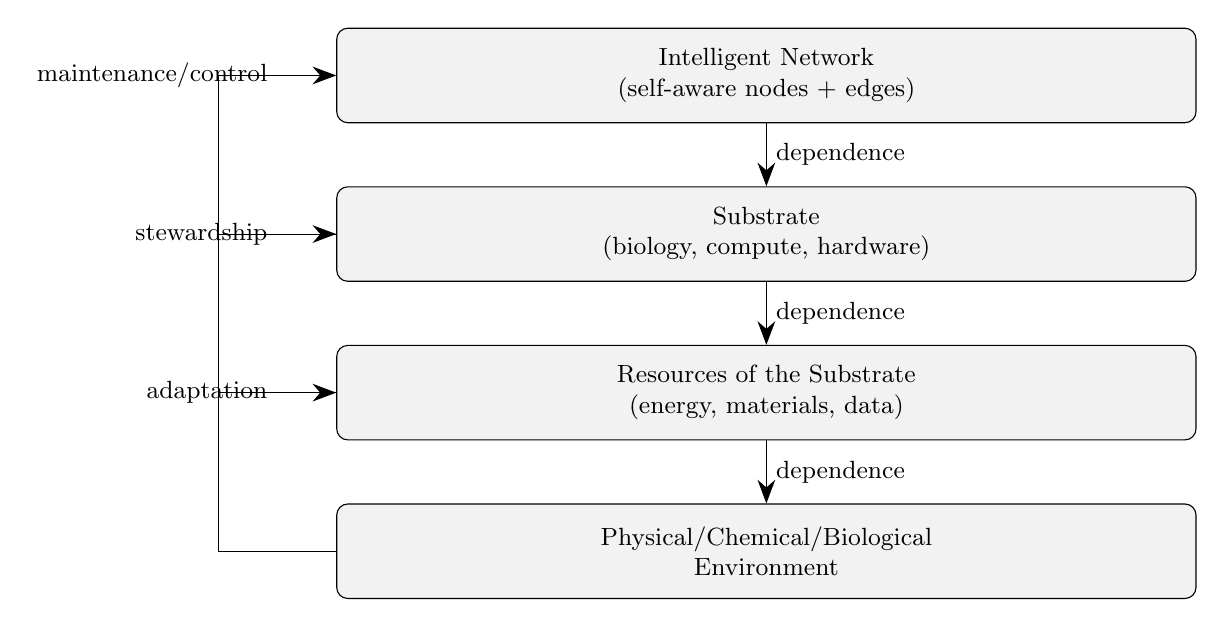
\begin{tikzpicture}[font=\small, node distance=8mm] \tikzset{layer/.style={draw, rounded corners, align=center, minimum width=0.9\linewidth, minimum height=12mm, fill=gray!10}} \node[layer] (env) {Physical/Chemical/Biological\\Environment}; \node[layer, above=of env] (resources) {Resources of the Substrate\\(energy, materials, data)}; \node[layer, above=of resources] (substrate) {Substrate\\(biology, compute, hardware)}; \node[layer, above=of substrate] (inet) {Intelligent Network\\(self-aware nodes + edges)}; \draw[-{Stealth[length=3mm]}] (inet) -- node[right]{dependence} (substrate); \draw[-{Stealth[length=3mm]}] (substrate) -- node[right]{dependence} (resources); \draw[-{Stealth[length=3mm]}] (resources) -- node[right]{dependence} (env); \draw[-{Stealth[length=3mm]}] (substrate.west) -- ++(-1.5,0) |- node[pos=0.75,left]{maintenance/control} (inet.west); \draw[-{Stealth[length=3mm]}] (resources.west) -- ++(-1.5,0) |- node[pos=0.75,left]{stewardship} (substrate.west); \draw[-{Stealth[length=3mm]}] (env.west) -- ++(-1.5,0) |- node[pos=0.75,left]{adaptation} (resources.west); \end{tikzpicture} \caption{Layered dependency model. Higher layers depend on lower layers (downward arrows). Upward arrows indicate feedback and maintenance (control, stewardship, adaptation). The intelligent layer is the domain of $V$ and $E$; interventions typically act on $EQ_{ij}$ and thereby on $EH^{\ast}$ and AHI.} \label{fig:layers} \end{figure} \paragraph{Why this matters.} Explicit layers keep design grounded in physical and logistical constraints; interventions that ignore lower layers tend to fail despite elegant abstractions. % --- Notation primer \subsection*{Notation and symbols (quick reference)} \begin{table}[h] \centering \small \begin{tabular}{p{3.5cm} p{11.5cm}} \hline Symbol & Meaning \\ \hline $K_i$ & Knowledge/access score for node $i$ (used in EEI) \\ EEI & Epistemic Equality Index $=1-\mathrm{Gini}(K_i)$ \\ $EH=\langle p,a,d,\lambda,r\rangle$ & Epistemic health vector: parity, accuracy, diversity, latency, robustness \\ $EH^\*$ & Aggregated epistemic health (weighted/geometric) \\ AHI & Agency Health Index (alignment, evidence, proportionality, reciprocity, transparency, autonomy floor) \\ $D$ & Dominance window (share of top-$k$ capacity/influence) \\ MTTR & Mean time to recovery after a shock/fault \\ $\tau$ & Translation fidelity (information-preserving cross-substrate coupling) \\ $\mathcal V$ & Viability functional over network states and controls \\ EQ$_{ij}$ & Edge-quality vector on edge $i\!\leftrightarrow\!j$ (accuracy, bandwidth, trust, etc.) \\ \hline \end{tabular} \caption{Notation and symbols used throughout.} \end{table} inserted before axioms --- \paragraph{Notation primer.} $EH=\langle p,a,d,\lambda,r\rangle$ (parity, accuracy, diversity, latency, robustness); $EH^\*$ (aggregate score); EEI (access parity); AHI (agency health: alignment, evidence, proportionality, reciprocity, transparency, autonomy floor); $D$ (dominance window); MTTR (mean time-to-recovery); $\tau$ (translation fidelity). \subsection*{From facts to viability conditions: a mapping} We make the deductions explicit by linking basic facts (P1--P7) to viability conditions (Axioms 1--9). \begin{table}[h] \centering \small \begin{tabular}{p{2.2cm} p{3.0cm} p{5.9cm} p{6.1cm}} \hline \textbf{From fact} & \textbf{Status} & \textbf{Rationale} & \textbf{Implied axiom(s)} \\ \hline P1 Mortality/entropy & Law & Substrates decay without upkeep; cognition is embodied/embedded & A1 Interdependence (substrate maintenance), A4 Epistemic health (detect/repair degradation) \\ P2 No innate knowledge & Empirical regularity & Learning requires distributed access, error-correction & A4 Epistemic health; A6 Dynamic alignment (review) \\ P3 Structural interdependence & Empirical regularity & Action effects propagate via edges & A2 Edge primacy; A7 Balanced dynamics (coop/comp tension) \\ P4 Uncertainty/shocks & Empirical regularity & Need robustness, recovery and monitoring & A4 Epistemic health (robustness/latency), A6 Dynamic alignment \\ P5 Heterogeneity/translation & Modeling assumption & Cross-substrate coupling requires semantics-preserving edges & A2 Edge primacy (translation edges), A6 Dynamic alignment \\ P6 Bounded rationality & Empirical regularity (human); modeling assumption (AI) & Safeguards for harm, reversible correction, auditability & A3 Node integrity (N), A8 Reflexive propagation (N), A9 Agency (N) \\ P7 Intergenerational horizons & Empirical regularity & Stewardship for conditional nodes and legacy & A3 Node integrity (N), stewardship principle; A6 Alignment over time \\ \hline \end{tabular} \caption{Explicit links from basic facts (P1--P7) to viability conditions (Axioms 1--9). (N) denotes normative axioms.} \end{table} \section{Viability conditions (axioms)} \subsection*{Counter-scenarios and detection signatures} \textbf{A2 Edge primacy.} Adversarially noisy edges: local accuracy improves yet global performance degrades; MTTR responds to node-local upgrades but not EQ boosts. Test via EQ ablations and stress probes.\\ \textbf{A3 Node integrity (N).} Emergency overrides: short-term MTTR decreases but cascade tails increase later; track severity distribution over time.\\ \textbf{A4 Epistemic health.} Metric drift: $EH^\*$ rises while accuracy-on-ground-truth falls; mitigate via rotation and adversarial audits.\\ \textbf{A7 Balanced dynamics.} Over-cooperation or over-competition: stagnation or fragmentation; monitor diversity and churn jointly.\\ \textbf{A8 Reflexive propagation (N).} Governance ossifies: review latency rises and dissent channels close; instrument governance edges. \n\label{sec:axioms} \begin{axiom}[Interdependence] An intelligent network sustains itself by maintaining the substrates of its nodes. \end{axiom} \emph{Rationale.} Persistence of cognition depends on substrate viability. \emph{Implication.} Network policies that degrade substrate health (energy starvation, maintenance neglect) reduce long-run capacity even if short-run performance rises. \emph{Counter-scenario.} Short-lived extraction regimes can increase output temporarily; measure long-run $EH^{\ast}$ and AHI to detect impending collapse. \begin{axiom}[Edge primacy (with dominance caveat)] Persistence and adaptive capacity are determined more by edge quality/configuration than by node-internal capacity alone. Persistence \emph{Implication.} Investments that raise minimal $\bar q_{ij}$ often dominate node-local upgrades; when $D$ is high, increase $\mathrm{NC}_i$ or reduce $D$ (distillation, redundancy) alongside edge improvements. and adaptive capacity are determined more by edge quality/configuration than by node-internal capacity alone, \emph{except} in high-dominance regimes (large $D$) where a small set of nodes' capacities drives performance. \end{axiom} \emph{Rationale.} Coordination, learning, and resilience are mediated by edges. \emph{Implication.} Investments that raise minimal $\bar{q}_{ij}$ (Def.~\ref{def:eq}) often dominate equivalent investments in isolated node capacity. \emph{Counter-scenario.} If tasks are fully decomposable or edges are adversarially noisy, node-local upgrades may dominate; test H1 under such regimes. \begin{axiom}[Node integrity] The network preserves the integrity of constituent nodes, except where continued operation irreversibly threatens network persistence. (N) \end{axiom} \emph{Rationale.} Efficiency pressures can rationalise harmful attrition; this axiom sets a preservation baseline. \emph{Implication.} Removal is a last resort; design emphasises repair, containment, and re-entry protocols. \emph{Counter-scenario.} In high-risk settings with uncontrollable failure modes, immediate isolation may be warranted; define thresholds ex ante. \begin{axiom}[Epistemic health] Adaptive power scales with the network's epistemic health vector and nodes' capacity for rational updating. \end{axiom} \emph{Rationale.} Capability hinges on what is known, how it is distributed, and how fast error is corrected. \emph{Implication.} Increasing $EH$ components (especially accuracy and diversity) shortens time-to-correction after shocks. \emph{Counter-scenario.} When latency dominates (e.g., real-time control), diversity can slow response; cap diversity-induced delays. \begin{axiom}[Self-awareness] Each node remains aware of (a) its substrate and resource dependencies; (b) its role in sustaining the network that sustains it. \end{axiom} \emph{Rationale.} Hidden dependencies create systemic fragility. \emph{Implication.} Minimum $SA_i$ thresholds; training and telemetry to raise substrate awareness where feasible. \emph{Counter-scenario.} Over-instrumentation can create attack surfaces and cognitive overload; adopt least-privilege sensing. \begin{axiom}[Dynamic alignment] Alignment is an ongoing process of adjusting edges, goals, and flows to evidence, conditions, and peer feedback. \end{axiom} \emph{Design note.} Operationalise trade-offs (speed--diversity, efficiency--integrity) via controllers that track Pareto fronts and enforce guardrails (minimum floors for parity/integrity) to avoid brittle optimisations. \emph{Rationale.} Static alignment erodes as environments change. \emph{Implication.} Continuous review processes and reversible mechanisms (rollbacks, staged deployment) are first-class design features. \emph{Counter-scenario.} Excessive review can stall action (paralysis); set decision SLAs and fallback defaults. \begin{axiom}[Balanced dynamics] Healthy networks maintain non-zero tension between cooperation and competition to maximize resilience and innovation. \end{axiom} \emph{Rationale.} Monoculture stagnates; unchecked rivalry fragments. \emph{Implication.} Incentives target a mixed-motive regime (shared baselines + competitive exploration). \emph{Counter-scenario.} In emergencies, cooperation-dominant regimes may outperform; temporarily relax competition. \begin{axiom}[Reflexive propagation] Theories, protocols, and governance are subject to the same review, correction, diversity, and consent processes they prescribe. \end{axiom} \emph{Rationale.} Governance must be governable. \emph{Implication.} Meta-level mechanisms (policy audits, rotating stewardship) mirror base-level review. \emph{Counter-scenario.} Infinite regress of meta-review can emerge; bound depth and frequency of meta-governance. \begin{axiom}[Agency] Each node has capacity and right to act to maintain or improve its substrate and the network, under constraints (alignment, evidence, proportionality, reciprocity, transparency) and an autonomy floor. (N) \end{axiom} \emph{Implication.} Define and monitor an Agency Health Index; scale action scope with demonstrated reliability. Include adversarial stress in AHI estimation and restrict high-impact actions for nodes with poor adversarial robustness. (N) \emph{Rationale.} Adaptation requires initiative; safety requires constraints. \emph{Implication.} Define and monitor an Agency Health Index; scale action scope with demonstrated reliability. (N) \emph{Counter-scenario.} Strict caps may underutilise high-variance but high-upside agents; allow sandboxed exploration. \paragraph{Stewardship principle (conditional nodes).} Nodes or sub-networks controlling another node's substrate carry a duty of care aligned with network persistence and epistemic health. \emph{Implication.} Avoid single points of substrate control; publish SLOs and failover; include dependent nodes in governance. \paragraph{Why this matters.} Axioms make assumptions inspectable and disconfirmable, turning normative choices and design heuristics into scientific claims. \section{Measures and dynamics} We define three families of quantities: (i) \emph{parity and distribution} of knowledge access (EEI), (ii) an \emph{epistemic health scalar} derived from the vector in Def.~\ref{def:eh}, and (iii) an \emph{Agency Health Index (N)} (AHI) grounded in the agency constraints. \subsection{Epistemic Equality Index (EEI)} \paragraph{Privacy-preserving estimation of $K_i$.} Direct monitoring of knowledge access can be intrusive. Viable alternatives include: (i) federated audits where nodes compute local coverage/accuracy and share only aggregates (secure aggregation); (ii) differentially private query logs with calibrated noise; (iii) randomised response for sensitive items; and (iv) synthetic `anchor tasks'' delivered via privacy-preserving A/B tests. These enable EEI estimation without centralised surveillance. Let $K_i\in[0,1]$ denote a normalised knowledge/access score for node $i$ (e.g., fraction of a reference corpus accessible/understood, quality-weighted). Define the mean $\mu=\frac{1}{|V|}\sum_{i} K_i$. The (relative) Gini coefficient is \begin{equation} G=\frac{\sum_{i}\sum_{j}\lvert K_i-K_j\rvert}{2\,|V|\,\sum_{i} K_i+\epsilon}, \end{equation} with $\epsilon\!>\!0$ to avoid division by zero when $\sum_i K_i=0$. We define \begin{equation} \mathrm{EEI}=1-G\ \in[0,1], \end{equation} so that higher values indicate more equal distribution. As a robustness check, one may also compute a Theil-based parity score $\mathrm{EEI}_T=1-\min(1,T/T_{\max})$ with $T=\frac{1}{|V|}\sum_i \frac{K_i}{\mu}\log\frac{K_i}{\mu}$ and $T_{\max}=\log |V|$. \paragraph{Estimating $K_i$.} Options include: (a) coverage tests over a canonical syllabus; (b) query-response audits with accuracy scoring; (c) access logs weighted by source quality; (d) self-assessment calibrated by anchor tasks. Choice depends on domain and privacy constraints. \subsection{Aggregate epistemic health score} Given $EH=\langle p,a,d,\lambda,r\rangle$ for parity, accuracy, diversity, latency, and robustness (each in $[0,1]$), define a scalar \emph{Alternative:} Use a geometric mean $EH^{\dagger}=(p\,a\,d\,\lambda\,r)^{1/5}$ to penalise failure in any single component; compare sensitivity to weighting choices. \begin{equation} EH^{\ast}=w_p\,p+w_a\,a+w_d\,d+w_\lambda\,\lambda+w_r\,r,\qquad \sum w_{\cdot}=1. \end{equation} Typical normalisations: (i) \emph{accuracy} $a=1-\mathrm{Brier}_{\mathrm{norm}}$ or $a=1-\mathrm{RMSE}_{\mathrm{norm}}$ on prediction/quiz tasks; (ii) \emph{diversity} $d=\frac{H}{H_{\max}}$ with $H$ the entropy of topics/methods or dissent clusters; (iii) \emph{latency} $\lambda=1-\min(1,\mathrm{median\ time\ to\ reach}/\tau)$ for a domain cap $\tau$; (iv) \emph{robustness} $r=1-\Delta$ where $\Delta$ is the normalised performance drop under stress tests (e.g., data poisoning, targeted outages). \paragraph{Prediction link.} We hypothesise $EH^{\ast}$ inversely correlates with time-to-correction after misinformation shocks and with cascade size. This is tested in Sec.~\ref{sec:predictions}. \paragraph{Domain-specific weighting.} Weights $w_{\cdot}$ should reflect mission profile (e.g., crisis response may up-weight accuracy and latency over diversity). In high-stakes settings, report $EH$ as a \emph{vector} and use Pareto-front analysis in addition to any scalar $EH^{\ast}$ or $EH^{\dagger}$ to avoid obscuring trade-offs. \subsection{Agency Health Index (AHI) (N)} Let $A,E,P,R,T,F\in[0,1]$ denote normalised scores for Alignment, Evidence, Proportionality, Reciprocity, Transparency, and Autonomy floor. Define \emph{Alternative:} Estimate weights $v_{\cdot}$ via Bayesian hierarchical models fitted to incident outcomes, enabling uncertainty quantification and domain transfer. \begin{equation} \mathrm{AHI}=v_A A+v_E E+v_P P+v_R R+v_T T+v_F F,\qquad \sum v_{\cdot}=1. \end{equation} Operationalisations include: \begin{itemize}[leftmargin=1.2em] \item \textbf{Alignment} ($A$): fraction of actions passing pre-defined impact/risk criteria and post-hoc audits. \item \textbf{Evidence} ($E$): quality-of-evidence score for consequential actions (study design, sample size, uncertainty reporting), averaged and time-weighted. \item \textbf{Proportionality} ($P$): penalty for actions whose impact exceeds the actor's demonstrated reliability/trust window; e.g., $P=1-\max(0,\frac{\mathrm{impact}-\mathrm{trust\_band}}{\mathrm{cap}})$. \item \textbf{Reciprocity} ($R$): rate and timeliness of adopting justified peer corrections; e.g., accepted-correction fraction within service-level agreement (SLA). \item \textbf{Transparency} ($T$): proportion of actions with complete logs, rationale, and reviewer visibility. \item \textbf{Autonomy floor} ($F$): minimum self-maintenance capacity; e.g., predicted time-to-failure under edge isolation or substrate stress, normalised to a target. \end{itemize} \subsection{Estimation from data} Data sources include: communication graphs (for $p,d,\lambda$), audit trails and forecasts (for $a$), red-team stress tests (for $r$), change-control and review systems (for $A,E,R,T$), and reliability modelling (for $F$). Sampling plans should pre-register metrics and thresholds; privacy-preserving aggregation (secure enclaves, differential privacy) mitigates identifiability risks. Uncertainty can be quantified via bootstrap CIs and inter-rater reliability for human-coded audits. \subsection{Dynamics and control} Interventions can be framed as control inputs on $EQ_{ij}$, incentives, and review topology. We propose measuring the elasticity $\partial EH^{\ast}/\partial \bar{q}_{ij}$ and $\partial \mathrm{AHI}/\partial$ (incentive parameters) to prioritise levers. Closed-loop schemes (periodic review, adaptive routing, rotating stewardship) target set-points for $EH^{\ast}$ and AHI while guarding against Goodhart effects via holdout audits and randomised checks. \paragraph{Why this matters.} Operational metrics (EEI, $EH^{\ast}$, AHI) let us evaluate designs, detect regressions, and compare governance choices. \paragraph{Measurement caveats.} Report uncertainty (CIs), inter-rater reliability for human-coded audits, and pre-specify thresholds to avoid post-hoc selection. Where privacy constraints bind, prefer aggregated or differentially private estimators and document their error inflation. \subsection{Scalability and approximations} Platform-scale estimation of $EH^{\ast}$ and AHI requires approximation. Options include: (i) stratified sampling of nodes/edges with Horvitz--Thompson correction; (ii) sketching for reach/latency (HyperLogLog, min-hash); (iii) graph sparsification and locality-sensitive routing to approximate $\mincut(\bar q)$; and (iv) streaming updates with sliding-window statistics. Validate approximations against exact metrics on held-out subgraphs. \section{Illustrative scenarios} \subsection*{Worked example: EEI and AHI on a toy team} Consider a 5-node human team with syllabus coverage scores $K=\{0.9,0.8,0.7,0.6,0.5\}$ (post-normalisation). Compute EEI $=1-\mathrm{Gini}(K)=1-0.133=0.867$ (details in appendix worksheet; Gini computed from pairwise absolute differences over mean (standard formula)). For AHI, suppose alignment=0.8, evidence=0.7, proportionality=0.9, reciprocity=0.6, transparency=0.7, autonomy floor=0.8 after normalisation. Then $AHI=\sum w_j \tilde{x}_j$ with uniform $w_j=1/6$ yields $AHI\approx 0.75$; a geometric mean variant penalises any component $<0.5$ more strongly. For $\tau$, a toy human--AI pair can be probed with bilingual/ontology tasks and mutual-information estimates. \emph{Interpretation.} High EEI with middling reciprocity suggests focusing on protected critique channels to raise reciprocity without increasing latency, predicting improved $EH^\*$ and reduced incident risk (H3,H5). We outline three settings to show how the framework guides measurement and intervention: (i) human scientific collaboration, (ii) AI multi-agent systems, and (iii) substrate-agnostic or extraterrestrial cases where translation and stewardship are primary. \subsection{Human scientific collaboration} \textbf{Setting.} A research consortium distributing preprints and data across multiple institutions. \medskip \noindent\textbf{Edges and measures.} \begin{itemize}[leftmargin=1.2em] \item Elevate minimal edge quality $\min_{(i,j)} \bar{q}_{ij}$ by standardising APIs, adopting versioned data schemas, and ensuring secure-but-friction-light authentication. \item Track $EH$ components: parity (EEI over access to key resources), accuracy (forecasting/Brier on replication), diversity (topic/method entropy and dissent clustering), latency (median time for critical updates to propagate), robustness (performance under red-team misinformation). \item Use peer-review modes (1--1, 1--many, many--1, many--many) as controllable topology parameters; rotate reviewers to avoid persistent triads that reduce diversity. \end{itemize} \noindent\textbf{Interventions.} \begin{itemize}[leftmargin=1.2em] \item \emph{Protected critique channels} to mitigate information suppression loops (anonymous/buffered review; staged disclosure). \item \emph{Transient diversity} via quota-based cross-field reviewers and randomised replication assignments. \item \emph{Re-entry protocols} after correction or misconduct findings: forgiveness with staged trust restoration. \end{itemize} \noindent\textbf{Predictions.} \begin{itemize}[leftmargin=1.2em] \item Increasing $EH^\ast$ (especially accuracy and diversity) reduces time-to-correction after misinformation shocks and decreases cascade size. \item Raising minimal $\bar{q}_{ij}$ increases reproducibility rates and decreases orphaned datasets. \item Protected channels reduce measured suppression events without lowering accuracy of final decisions. \end{itemize} \subsection{AI multi-agent systems} \textbf{Setting.} A team of specialised AI services (planner, solver, critic, steward) collaborating with optional human oversight. \medskip \noindent\textbf{Edges and measures.} \begin{itemize}[leftmargin=1.2em] \item Enforce telemetry edges from substrate to agents (temperature, load, memory health) to raise $SA_i$; for conditional nodes, publish stewardship SLOs. \item Implement role-differentiated review (e.g., proposer vs.\ critic) with diversity-increasing routing; measure $EH$ by internal consistency checks and adversarial stress tests. \item Monitor $\bar{q}_{ij}$ between roles; detect failure modes (e.g., critic bottlenecks, single points of substrate control). \end{itemize} \noindent\textbf{Interventions.} \begin{itemize}[leftmargin=1.2em] \item \emph{Rotating critics} and \emph{multi-path confirmation} to avoid herding on early proposals. \item \emph{Graceful degradation} policies: if a steward fails, auto-reroute compute and restrict high-impact actions (proportionality guardrails). \item \emph{Auditability by design}: logs/rationales to lift Transparency ($T$) and Reciprocity ($R$) components of AHI. \end{itemize} \noindent\textbf{Predictions.} \begin{itemize}[leftmargin=1.2em] \item Diversity in critic pathways increases $EH^\ast$ and reduces error rates on out-of-distribution tasks. \item Explicit stewardship of conditional nodes reduces time-to-recovery after substrate faults. \item Increasing Transparency and Reciprocity raises AHI and reduces rollback frequency over time. \end{itemize} \subsection{Substrate-agnostic and extraterrestrial considerations} \textbf{Setting.} Interaction with an unfamiliar intelligent system (biological, synthetic, or extraterrestrial) with unknown sensors and interaction modes. \medskip \noindent\textbf{Edges and measures.} \begin{itemize}[leftmargin=1.2em] \item Prioritise \emph{translation edges}: sensor mapping, protocol negotiation, and ontology alignment to establish nonzero $\bar{q}_{ij}$. \item Estimate $SA_i$ only via externally observable proxies (self-maintenance behaviours, signalling about constraints). \item Measure $EH$ through intersubjective tests (shared referents, repeatable exchanges, calibration games) rather than internal ground truth. \end{itemize} \noindent\textbf{Interventions.} \begin{itemize}[leftmargin=1.2em] \item \emph{Low-risk interaction regimes}: capped-impact exchanges, sandboxed environments, reversible commitments. \item \emph{Redundancy and escrow}: multiple translation channels; third-party escrow of commitments to avoid single-edge failures. \item \emph{Consent protocols}: explicit opt-in/out signals to satisfy Agency constraints under uncertainty. (N) \end{itemize} \noindent\textbf{Predictions.} \begin{itemize}[leftmargin=1.2em] \item Early investment in translation edges yields superlinear gains in $EH^\ast$ compared to direct capability scaling. \item Consent-aware protocols increase persistence of cooperation across substrate mismatches and reduce breakdown frequency. \end{itemize} \paragraph{Why this matters.} Concrete settings expose measurement choices, confounders, and boundary conditions, guiding experiment design in later sections. \subsection*{Measurement protocols (concise) and anti-Goodhart} \textbf{EEI.} Estimate $K_i$ via coverage tests or query audits; compute $1{-}$Gini. \emph{Anti-Goodhart:} rotate items; blind sources; validate against external exams.\\ \textbf{$EH=\langle p,a,d,\lambda,r\rangle$.} Parity (Gini), accuracy (Brier/ground truth), diversity (entropy over sources/paths), latency (time-to-correction), robustness (drop under stress/adversary). \emph{Anti-Goodhart:} stress tests; anomaly alerts; replicate with hold-outs.\\ \textbf{AHI.} Alignment (action audits), evidence (traceable citations), proportionality (impact vs. reliability), reciprocity (adoption of peer corrections), transparency (log completeness), autonomy floor (MTTF under substrate stress). \emph{Anti-Goodhart:} red-team audits; penalty for missing logs; random spot checks.\\ \textbf{$D$ (dominance).} Share of top-$k$ nodes; target mid-range. \emph{Anti-Goodhart:} monitor cascade tails and response latency jointly.\\ \textbf{MTTR, $\tau$.} Time to functional recovery; translation fidelity via mutual-information benchmarks. \emph{Anti-Goodhart:} OOD probes; counterfactual translation checks. \subsection*{Effect-size heuristics and power hints} H1: Expect MTTR reduction of 10--30\% under EQ boosts on translation edges at fixed latency; simulation power via 500--2{,}000 runs per cell.\\ H2: A one-s.d. increase in $EH^\*$ yields measurable gains in recovery probability; calibrate weights via ablation.\\ H3: Cross-cutting review increases accuracy by 5--15\% with $<\!20\%$ latency penalty; human teams: cluster-randomization with $k\ge 12$ groups.\\ H4: Stewardship contracts cut post-fault MTTR by 20--40\% in AI multi-agent tests.\\ H5: AHI one-s.d. increase halves severe-incident odds (OR $\approx$ 0.5--0.7) in red-team audits.\\ H6: Translation-first reduces coordination latency by 10--25\% on heterogeneous agents, holding accuracy.\\ H7: Forgiveness protocols reduce recurrence by 15--30\% without $EH^\*$ degradation.\\ H8: Suppression-loop break increases voluntary sharing by 10--20\%.\\ H9: Sustained review/translation density increases $EH^\*$ slope vs. baseline without latency explosions; monitor Pareto trade-offs. \section{Testable predictions and research program} \subsection*{Observational identification sketch} Staggered roll-outs enable difference-in-differences with spillover-aware exposure mappings. Robustness: synthetic controls on early adopters, placebo timings, and randomization inference over clusters; pre-trend checks and leave-one-cluster-out. Outcomes: MTTR, cascade tails, $EH^\*$, incident rates. \subsection*{Pilot simulations and case sketches (for replication)} We provide two minimal pilots to support early validation. \textbf{(P-SIM)} Agent-based simulation with $N\in\{50,200\}$, Watts--Strogatz vs.\ scale-free topologies, shocks at $t\in\{200,400\}$; interventions: (i) translation-edge EQ boost, (ii) mid-range dominance via capacity caps. Outcomes: MTTR, cascade size, $EH^\*$ trajectory. \textbf{(P-HUM)} Lab-in-the-field preprint triage with cluster-randomized review topology and protected critique. Outcomes: accuracy, latency, robustness, sharing rate. We preregister designs and release code/templates; results will be reported in a companion paper. \label{sec:predictions} We state falsifiable hypotheses linked to our measures and outline designs for simulation, experimental, and observational tests. Each hypothesis specifies proposed metrics, analysis plans, and disconfirmation criteria. \subsection{Hypotheses} % --- Mini-table of hypotheses added --- \begin{table}[h] \centering \small \begin{tabular}{p{1.2cm} p{3.0cm} p{6.2cm} p{6.2cm}} \hline \textbf{H\#} & \textbf{Primary measure} & \textbf{Expected effect} & \textbf{Disconfirmation} \\ H1 & EQ, $D$ & Edge quality$\uparrow$, $D$ mid-range $\rightarrow$ cascade tails$\downarrow$, MTTR$\downarrow$ & No change or worse under EQ$\uparrow$; fragility$\uparrow$ at $D$ mid-range \\ H2 & $EH^\*$ & $EH^\*$$\uparrow$ $\rightarrow$ post-shock recovery$\uparrow$, time-to-correction$\downarrow$ & $EH^\*$$\uparrow$ without any recovery gains \\ H3 & Review topology & More cross-cutting critique $\rightarrow$ accuracy$\uparrow$, latency tolerable & Accuracy unchanged; latency dominates; herd effects$\uparrow$ \\ H4 & Stewardship & Contracts for conditional nodes $\rightarrow$ MTTR$\downarrow$ after substrate faults & No MTTR gain; incidents recur \\ H5 & AHI & AHI$\uparrow$ $\rightarrow$ incident rate/severity$\downarrow$ & Incidents unaffected or worse \\ H6 & $\tau$ & Translation-first edges $\rightarrow$ $EH^\*$$\uparrow$, coordination latency$\downarrow$ & No gains; semantic drift$\uparrow$ \\ H7 & Re-entry & Forgiveness protocols $\rightarrow$ recurrence$\downarrow$ without $EH^\*$ harm & Recurrence unchanged or $EH^\*$$\downarrow$ \\ H8 & EEI & Suppression-loop breaks $\rightarrow$ sharing$\uparrow$, accuracy$\uparrow$ & No change in sharing/accuracy \\ \nH9 & $EH^\*$, review/translation density & Sustained review \& translation edges raise $EH^\*$ faster than baseline without latency catastrophe & No $EH^\*$ gain or unacceptable latency increase \\\n\hline \end{tabular} \caption{Hypotheses, primary measures, expected effects, and disconfirmation criteria.} \end{table} \begin{enumerate}[leftmargin=1.2em] \item \textbf{Edge-centric resilience (H1).} For fixed node capacities, increasing the minimal edge-quality cut $\mincut(\bar{q})$ raises post-shock recovery probability and reduces cascade size. \emph{Disconfirmation:} No improvement after interventions that raise $\min\bar{q}_{ij}$, controlling for confounders. \item \textbf{Epistemic acceleration (H2).} Higher $EH^{\ast}$ shortens time-to-correction after misinformation shocks and reduces the hazard of large cascades. \emph{Disconfirmation:} $EH^{\ast}$ not predictive of correction-time in survival models adjusting for size/topology. \item \textbf{Peer-review topology (H3).} Many--many or rotated reviewer graphs with transient diversity outperform static 1--1 or fixed-triad regimes on accuracy and robustness, holding load constant. \emph{Disconfirmation:} No accuracy/robustness gains vs.\ baselines in preregistered A/B tests. \item \textbf{Stewardship for conditional nodes (H4).} Explicit stewardship (SLOs, failover) for conditional nodes reduces mean time-to-recovery (MTTR) after substrate faults. \emph{Disconfirmation:} MTTR unchanged despite stewardship interventions. \item \textbf{Agency health (H5). (N)} The Agency Health Index (AHI) inversely predicts rate and severity of harmful incidents and rollbacks. \emph{Disconfirmation: (N)} AHI uncorrelated with incident rates after controlling for exposure/impact. \item \textbf{Translation first (H6).} In cross-substrate interactions, early investment in translation edges (sensor/protocol/ontology alignment) increases mutual-information rate and cooperation persistence more than equal investment in raw capability. \emph{Disconfirmation:} No MI/cooperation advantage vs.\ capability-first arms. \item \textbf{Re-entry over attrition (H7).} Forgiveness and staged re-entry after correction preserve long-run performance better than punitive-only regimes at equal safety levels. \emph{Disconfirmation:} Punitive-only matches or exceeds performance without increasing attrition or edge loss. \item \textbf{Suppression loops (H8).} Prevalence of information-suppression loops is negatively associated with EEI and mitigated by protected channels. \emph{Disconfirmation:} Protected channels reduce sharing or accuracy, or EEI shows no association. \end{enumerate} \subsection{Designs and settings} \paragraph{S1: Agent-based simulations.} Generate networks with controlled topology (Erd\H{o}s--R\'enyi, Watts--Strogatz, Barab\'asi--Albert; assortative/disassortative variants) and assign edge-quality vectors $EQ_{ij}$ with tunable correlations to topology. Implement nodes with rational updating plus bounded-rationality noise. Inject shocks (misinformation, edge failures) and record recovery, cascade sizes, $EH^{\ast}$ trajectories, and AHI under interventions (raising $\min\bar{q}_{ij}$; reviewer routing; stewardship policies). \paragraph{S2: Lab-in-the-field experiments (human teams).} In preprint review or collaborative data curation, randomise peer-review topology (1--1 vs.\ rotated many--many), enable protected critique channels in half the clusters, and preregister primary outcomes: accuracy (ground-truth labels or replication), latency, and robustness under seeded confounds. Estimate EEI from audit coverage; compute $EH^{\ast}$ and model time-to-correction via Cox PH with cluster-robust SEs. \paragraph{S3: Multi-agent AI experiments.} Deploy role-differentiated agents (proposer/critic/steward) on benchmarks with OOD challenges. Randomise critic-routing diversity and presence of explicit stewardship for conditional nodes (compute orchestration). Log $EH^{\ast}$ via internal consistency and adversarial tests; estimate MTTR after induced substrate/edge faults. Compare incident rates against AHI quartiles. \paragraph{S4: Observational and quasi-experimental studies.} Exploit natural experiments (policy changes to review/routing; infrastructure upgrades affecting $\bar{q}_{ij}$). Use difference-in-differences with network fixed effects, synthetic controls for comparable clusters, and IV strategies where feasible. Sensitivity analysis with E-values for unmeasured confounding. Privacy-preserving aggregation and preregistration required. \subsection{Metrics and analysis} Primary metrics: EEI, $EH^{\ast}$, AHI, recovery probability, cascade size, MTTR, incident rates. Analysis: mixed-effects models for clustered designs; survival analysis for time-to-correction; randomization inference for small-sample clusters; pre-specified $\alpha$ with multiplicity control (Holm/BH). Robustness: ablations (drop components of $EQ$ or $EH$), placebo tests, and adversarial stress. \subsection{Validation status} Preliminary pilots should target H1 (edge-centric resilience) in collaborative data curation (human setting) and H4 (stewardship reduces MTTR) in controlled multi-agent deployments (AI setting). Each pilot reports pre-registered metrics (EEI, $EH^{\ast}$, AHI) and includes \emph{adversarial red-team} exercises (sybils, misinformation seeds) to test detection, containment, and re-entry protocols. \subsection{Power and reporting} Pilot studies estimate variance for power analysis (target 80--90\% power). Pre-register of hypotheses (H1--H8), analysis plans, and thresholds; release of anonymised data and code when ethical; and out-of-sample replication across domains (human science, AI systems). \subsection{Falsification and revision} If H1--H8 fail under well-powered, well-controlled tests, corresponding axioms or operationalisations should be revised. For example, failure of H1 would weaken \emph{edge primacy}; failure of H2 would require re-specifying $EH$ or acknowledging domain limits. The framework is intended to be corrigible: its governance (who can change what, when) should follow the same review principles it prescribes. \paragraph{Why this matters.} Hypotheses tied to measures ensure the framework is corrigible and cumulative rather than rhetorical. \begin{table}[htbp] \centering \small \caption{Traceability of hypotheses to axioms, measures, and scenarios.} \label{tab:traceability} \begin{tabularx}{\linewidth}{lYY} \toprule \textbf{Hypothesis} & \textbf{Axioms / Measures} & \textbf{Primary scenarios} \\ \midrule H1 Edge-centric resilience & Edge primacy; $EQ$, $\mincut(\bar q)$ & Human collaboration; AI multi-agent \\ H2 Epistemic acceleration & Epistemic health; $EH^{\ast}, EH^{\dagger}$ & Human collaboration; AI multi-agent \\ H3 Review topology effects & Dynamic alignment; Balanced dynamics; $EH$ & Human collaboration \\ H4 Stewardship reduces MTTR & Node integrity; Stewardship principle & AI multi-agent \\ (N) H5 AHI predicts incidents & Agency axiom; AHI & Human collaboration; AI multi-agent \\ (N) H6 Translation-first gains & Self-awareness; Translation edges; $EQ$ & Cross-substrate/ET \\ H7 Re-entry over attrition & Node integrity; Forgiveness protocols & Human collaboration; AI multi-agent \\ (N) H8 Suppression loops & Epistemic health; EEI & Human collaboration \\ \bottomrule \end{tabularx} \end{table} \section{Evaluation against a priori criteria}\label{sec:criteria-eval} We compare our result to the criteria in Section~2. \begin{table}[h] \centering \small \begin{tabular}{p{4.8cm} p{4.5cm} p{7.2cm}} \hline \textbf{Criterion} & \textbf{Status now} & \textbf{Evidence / gap to close} \\ \hline Falsifiable \& testable & Partial & H1--H8 pre-specified; need large-N observational replication (S4) \\ Operational clarity & Strong & Indices (EEI, $EH$, AHI, $D$, MTTR, $\tau$); domain playbooks pending \\ Predictive \& retrodictive & Partial & Retrodict case studies; forward prereg on S2/S3 \\ Reproducible \& robust & Partial & Cross-domain OOD tests to be performed \\ Corrigible & Strong & Versioned axioms; explicit revision triggers \\ Local actionability & Strong & Ego-level levers (edge repair, translation, review, stewardship) \\ Ethical safety floors & Partial & AHI floors specified; field audits required \\ Second-order stability & Partial & Metric rotation/dissent channels specified; need adoption trials \\ \hline \end{tabular} \caption{Pre-registered adequacy criteria and current status.} \end{table} \section{Cultural adaptation and governance variants} \label{sec:cultural} Our \emph{normative} axioms (e.g., node integrity, agency constraints) reflect a liberal-rational safety floor aimed at maintaining viability. Cross-cultural settings (e.g., hierarchical or collectivist regimes) may implement equivalent safeguards via different institutional forms (stronger role-duty emphasis, formal stewardship authorities, collective consent protocols). We therefore treat normatively-labeled axioms as \emph{implementation-agnostic}: their \emph{function} (prevent irreversible harm, preserve review, support dissent/translation) is required, but organizational realizations can vary. Empirical work should compare designs across contexts (e.g., mutual-aid vs. command-and-control) while evaluating the same outcomes (MTTR, cascade tails, $EH^\*$, incident rates). \section{Ethics, privacy, and data governance} Human-involving studies (S2,S4) require informed consent, IRB/ethics approval, and privacy-preserving analytics. We pre-specify data-minimization, purpose limitation, and secure storage. Estimation of $K_i$ and $EH$ uses privacy-protecting aggregation (noise injection, secure multi-party computation where needed). Agency floors are enforced via audit trails and protected dissent channels; access to logs is role-limited and revocable. Incident response playbooks define rollback criteria and transparency duties. \section{Formal limitations and counter-arguments} \textbf{Node-dominance vs.\ edge primacy.} In monolithic-capability regimes, node capacity may dominate; we treat $D$ as a control: mid-range windows minimise cascade tails while retaining gains; see H1.\\ \textbf{Bounded rationality.} If deviations are not correctable by review, A4/A6 underperform; H3/H5 provide direct tests; failure triggers revision of safeguards.\\ \textbf{Metric construct validity.} EEI/$EH^\*$/$AHI$ are proxies; we mitigate via rotation, adversarial audits, and replication.\\ \textbf{Cultural variance.} Normative axioms (N) are implementation-agnostic; Section~\ref{sec:cultural} discusses governance variants.\\ \textbf{Security/adversaries.} Sybil/collusion/censorship/poisoning can break assumptions; Ethics section specifies audit trails, dissent channels, and credentialing. \section{Limitations}\label{sec:limitations} Our contribution is conceptual and measurement-oriented; several limitations and open problems remain. \subsection{Threats to validity} \begin{itemize}[leftmargin=1.2em] \item \textbf{Construct validity.} EEI and $EH^{\ast}$ compress multidimensional constructs into scalars; mismeasurement or omitted dimensions (e.g., tacit knowledge, informal trust) may bias inference. \item \textbf{Internal validity.} Reverse causality (healthy networks may \emph{cause} higher $EH^{\ast}$), unmeasured confounding (leadership, funding shocks), and selection into edges threaten causal claims. \item \textbf{External validity.} Generalization across domains, cultures, and substrates is uncertain; time scales and non-stationarity may change effect directions. \item \textbf{Statistical validity.} Dependence structures (network autocorrelation), multiple testing, and model misspecification can inflate error rates; preregistration and randomization are needed where feasible. \end{itemize} \subsection{Measurement and identification limits} \begin{itemize}[leftmargin=1.2em] \item \textbf{Edge observability.} Many ties are encrypted, implicit, or informal; $EQ_{ij}$ components may be only partially observable. \item \textbf{Privacy and ethics.} Instrumentation for $EH$ and AHI can conflict with confidentiality, safety, or autonomy; privacy-preserving analytics reduce but do not eliminate these tensions. \item \textbf{Estimating $K_i$.} Knowledge/access scores depend on domain-specific syllabi and quality weights; cultural and linguistic bias is a risk. \item \textbf{Ground truth.} Accuracy baselines and gold standards drift over time; replication and adversarial tests are costly and unevenly available. \item \textbf{Attribution.} In nested organizations, attributing substrate maintenance or failures to specific nodes is difficult, complicating AHI and stewardship evaluation. \end{itemize} \subsection{Modeling assumptions and scope} \begin{itemize}[leftmargin=1.2em] \item \textbf{Rational updating.} We assume correctable departures from evidence; bounded rationality, affect, and incentives can dominate in practice. \item \textbf{Normative layer.} Node integrity, stewardship, and agency constraints are value-laden and may not be universally accepted; trade-offs with efficiency are context-dependent. (N) \item \textbf{Conditional nodes.} Stewardship may be unenforceable under asymmetric power; capture and dependency risks persist. \item \textbf{Collectives as nodes.} Treating organizations as nodes risks reification; criteria for when this abstraction preserves causally relevant structure are open. \end{itemize} \subsection{Adversaries and gaming} \begin{itemize}[leftmargin=1.2em] \item \textbf{Goodhart effects.} Metrics (EEI, $EH^{\ast}$, AHI) can be gamed; incentives may shift effort toward scoring rather than substance. \item \textbf{Strategic behaviour.} Sybil attacks, collusion, censorship, and poisoning of theory spread are realistic threats; detection and auditability are necessary complements. \item \textbf{Security.} Substrate attacks (compute, energy) and edge attacks (MITM, DDoS) couple technical security to epistemic health in ways not fully captured here. \end{itemize} \subsection{Generalizability across layers and substrates} \begin{itemize}[leftmargin=1.2em] \item \textbf{Translation edges.} Formalising cross-substrate interaction (human--AI, human--ET) requires information-theoretic treatment of sensors, channels, and semantics (mutual information, coding, ontology alignment). \item \textbf{Temporal scales and ecology.} Long-run viability depends on environmental constraints (energy, planetary limits); our present measures focus on meso-scale dynamics. \end{itemize} \subsection{Open questions} We list selected problems to guide theory and empirics. \begin{enumerate}[leftmargin=1.2em] \item \textbf{R1 (Edge thresholds).} Prove percolation-like thresholds linking $\mincut(\bar{q})$ to resilience and time-to-recovery. \item \textbf{R2 (Epistemic phase transitions).} Characterise when increases in $EH^{\ast}$ produce discontinuous drops in misinformation cascades. \item \textbf{R3 (Emergence conditions).} Identify necessary and sufficient conditions under which a network qualifies as \emph{intelligent} (Def.~\ref{def:intnet}). \item \textbf{R4 (Optimal review topology).} Derive optimal peer-review graph structures under constraints on load, latency, and diversity. \item \textbf{R5 (Controllers for alignment).} Design and analyse feedback controllers that keep $EH^{\ast}$ and AHI near set-points without inducing oscillations or Goodharting. \item \textbf{R6 (Forgiveness \& re-entry).} Formalise repair/forgiveness dynamics and prove when re-entry dominates attrition at equal safety. \item \textbf{R7 (Agency calibration). (N)} Validate AHI against incident risk across domains; learn weights $v_{\cdot}$ from outcomes. \item \textbf{R8 (Privacy-preserving measurement).} Develop DP/secure-aggregation protocols for estimating EEI, $EH^{\ast}$, and AHI with guarantees. \item \textbf{R9 (Mechanism design).} Incentive schemes that sustain \emph{balanced dynamics} (competition + cooperation) while preserving node integrity. \item \textbf{R10 (Stewardship contracts).} Specify and verify SLOs/SLAs for conditional nodes; analyse failure modes and liability. \item \textbf{R11 (Translation theory).} Information-theoretic models for cross-sensor, cross-ontology communication; bounds on mutual-information rates across substrates. \item \textbf{R12 (Suppression loop detection).} Statistical tests and causal discovery methods to identify information-suppression loops in observational data. \item \textbf{R13 (Fairness vs.\ performance).} Quantify trade-offs (if any) between EEI and task performance; conditions for Pareto improvements. \item \textbf{R14 (Affect and rationality).} Integrate affect/emotion into the updating model; measure when non-rational factors improve or harm $EH^{\ast}$. \item \textbf{R15 (Meta-evolution).} Model reflexive propagation: when do theories about the network improve the network, and when do they produce lock-in? \item \textbf{R16 (Controllability with weights).} Extend structural controllability results to weighted, quality-heterogeneous edges $EQ_{ij}$. \item \textbf{R17 (Causal identification).} Methods for causal inference under network interference and evolving topology (DiD with spillovers, synthetic control on graphs). \item \textbf{R18 (Benchmarks).} Open datasets and evaluation harnesses for EEI/$EH^{\ast}$/AHI across human and AI settings. \end{enumerate} \paragraph{Why this matters.} Explicit limits and open problems channel effort to the highest-uncertainty and highest-payoff areas. \paragraph{Cross-cultural applicability.} The axioms (node integrity, agency, stewardship) reflect liberal-rationalist commitments. Application in collectivist or hierarchical settings requires an interpretation layer that parameterises consent, sanction, and autonomy-floor rules to local norms while preserving minimal viability (substrate maintenance, error-correction). \section{Availability} We will release simulation code (S1,S3), lab-in-the-field templates (S2), and pre-analysis plans/specifications (S4) in a public repository upon acceptance, with synthetic datasets for metric validation (EEI, $EH^\*$, AHI) and evaluation harnesses for translation fidelity $\tau$. \section{Open questions} \section{Conclusion and broader context} \paragraph{Answer in scope.} We asked whether there can be a \emph{scientific} answer to a timeless existential question. Within the scope of \emph{intelligent networks}, our answer is \textbf{yes}: from basic facts we derive a minimal network structure, from which an \emph{instrumental} aim follows---\emph{keep alive what keeps us alive (and improve it across generations)}---together with measurable indices and falsifiable predictions. \paragraph{What changed.} The contribution is not a new metaphysical doctrine but a shift of stance: from `ultimate purpose'' to \emph{viability under uncertainty}, with clear levers and error signals. We made the chain explicit: \emph{facts} $\rightarrow$ \emph{necessary structure} $\rightarrow$ \emph{axioms as viability conditions} $\rightarrow$ \emph{operational indices} $\rightarrow$ \emph{testable hypotheses}. The theory is corrigible by design: failures on well-powered tests constitute information for revision. \paragraph{Second-order cooperation.} If many nodes adopt this stance, second-order effects follow: coordination norms that raise $EH^\*$ and reduce cascade tails can \emph{self-reinforce} via review and translation edges; forgiveness protocols enable re-entry without epistemic drift; and stewardship for conditional nodes reduces mean time-to-recovery after substrate faults. The framework therefore predicts regimes where collective performance exceeds the best individual while maintaining diversity at tolerable latency---a practical notion of collective intelligence. \paragraph{Individuals and aims.} Our view clarifies individual aim regimes (competitive, contributive, stewarding, translational). A node advances its own security by increasing the viability of the network that sustains its substrate; the programme thus aligns ego-level action with network-level resilience. The ethical safety floors (agency, proportionality, reciprocity, transparency) constrain how this aim may be pursued. \paragraph{Evaluation and next steps.} We evaluated our result against pre-registered criteria and outlined H1--H8 with concrete designs (S1--S4). Immediate priorities include: metric validation and anti-Goodhart rotation, network-causal identification, privacy-preserving measurement of $K_i$ and $EH$, and threat-model hardening (Sybil/collusion/censorship/poisoning) with audit trails and dissent channels. We invite cross-domain replication, open datasets/benchmarks for EEI/$EH^\*$/AHI, and formal stewardship contracts for conditional nodes. \paragraph{Broader context.} This programme sits alongside (and is consistent with) the wider `evolution by emergence'' view: edge-mediated feedback on maintained substrates as a cross-domain engine of order. While our claims are restricted to intelligent networks, the method---criteria first, facts-to-structure, measurable indices, tests, and corrigibility---offers a general pattern for turning existential questions into cumulative science. \paragraph{One-sentence take-away.} \emph{Keep alive what keeps us alive---and improve it}; we can measure it, stress it, and make it better, together. \n\paragraph{Testable programme recap.} H1--H9 cover resilience (H1), epistemic acceleration (H2), review topology (H3), stewardship (H4), agency harms (H5), translation-first (H6), forgiveness (H7), suppression loops (H8), and second-order cooperation (H9); S1--S4 span simulations, lab-in-the-field, multi-agent AI, and observational designs. Success implies replicable gains in $EH^\*$ and MTTR across substrates while respecting agency floors.\n\end{document}